\documentclass{report}
\usepackage{caption}
\usepackage{setspace}
\usepackage{amsmath}
\usepackage{amssymb}
\usepackage{amsthm}
\usepackage{graphicx}
\usepackage{multirow}
\usepackage{geometry}
\usepackage{listings}
\usepackage{subfigure}
\usepackage{float}
\geometry{left=2.5cm,right=2.5cm,top=2.5cm,bottom=2.5cm}
\begin{document}
\begin{spacing}{1.3541667}
    
\section*{Question 2.from textbook}
{\bf (a)}\par
Now the weight of the pig becomes a function of $t$. 
And we want to find the velocity of this function, we need to find the differential of it. 
Then we get 

\begin{align*}
    \omega '(t)&=(\frac{800}{1+3e^{-\frac{t}{30}}})'\\
    &=\frac{80e^{-\frac{t}{30}}}{{1+3e^{-\frac{t}{30}}}^2}
\end{align*}

Then we set $t=0$, we can get 
\begin{align*}
    \omega '(0)=\frac{80}{16}=5(lbs)
\end{align*}

To ensure it is right, we can calculate that $w(0)=\frac{800}{4}=200$, 
and $w(1)=\frac{800}{1+3e^{-\frac{1}{30}}}=205.0415\approx 205$. 
So that $\Delta w \approx 5$.
So the pig is gaining about 5 lbs/day at $t=0$.

After that, we want to find how is the weight $\omega$ would happen 
when $t$ increases. 
I've written a project in MATLAB\@, in order to draw 2 picture of 
$t - \omega$ and $t - \omega '$ relationship. 

\begin{figure}[htbp]
    \centering
    \subfigure[Codes]{
        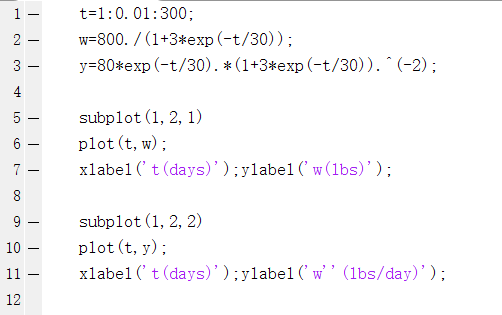
\includegraphics[scale=0.55]{figs/1(a)_1.jpg}
    }
    \hspace{0.1in}
    \subfigure[2 picture]{
        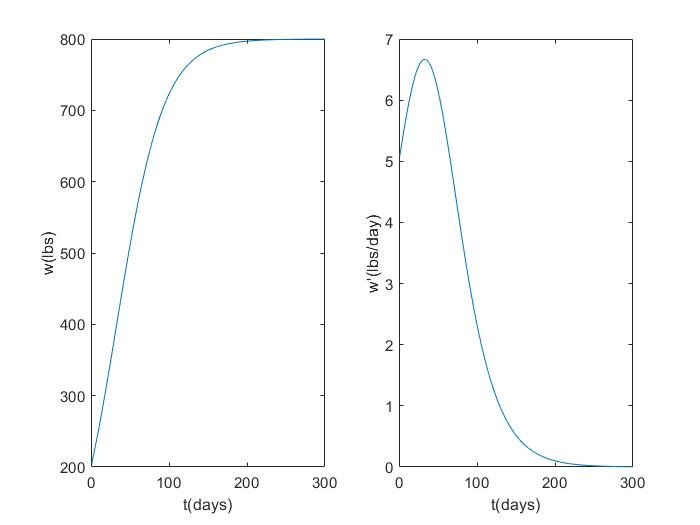
\includegraphics[scale=0.3]{figs/1(a)_2.jpg}        
    }
    \caption{Relationship between time $t$ and weight $\omega$}
\end{figure}

We can easily find that when $t \to \infty$ then $\omega \to 800$ and $\omega '\to 0$. 
And $\omega'$ is going upward firstly and then falling to 0 when $t$ becomes larger. 
Analying this, we can know that there is a fast grown of the weight of the pig $(\omega)$ 
and after that, we can sell the pig to gain the greatest profit. 

\newpage
{\bf (b)}\par
\hspace{-1.5em}{\bf Step 1. Ask the question}\par 
There three stages in step 1.

\vspace{0.5em}
\begin{tabular}{ll}
    {\bf Variables:}&$t$ = time (days)\\
    &$w$ = weight of pig (lbs)\\
    &$p$ = price for pigs (\$/lb)\\
    &$C$ = cost of keeping pig $t$ days (\$)\\
    &$R$ = revenue obtained by selling pig (\$)\\
    &$P$ = profit from sale of pig (\$)\\\vspace{-0.6em}\\
    {\bf Assumptions:}&$w=\frac{800}{1+3e^{-\frac{t}{30}}}$\\
    &$p=0.65-0.01t$\\
    &$C=0.45t$\\
    &$R=p\cdot w$\\
    &$P=R-C$\\
    &$t\geq0$\\\vspace{-0.6em}\\
    {\bf Objective:}&Maximize $P$
\end{tabular}

\vspace{1em}
\hspace{-1.5em}{\bf Step 2. Select the modeling approach}\par
We will model it as one-variable optimization problem. 
And we will use Newton method of one-variable to solve it. 

\vspace{1em}
\hspace{-1.5em}{\bf Step 3. Formulate the model}
Let $y=f(x)=P$, $x=t$. We can get 

\begin{align*}
    y&=f(x)\\
    &=(0.65-0.01x)(\frac{800}{1+3e^{-\frac{x}{30}}})-0.45x\\    
\end{align*}

And we can get the differential of $y$.

\begin{align*}
    f'(x)=-\frac{8}{1+3e^{-\frac{x}{30}}} + \frac{80(0.65-0.01x)e^{-\frac{x}{30}}}{{(1+3e^{-\frac{x}{30}})}^2}-0.45
\end{align*}

\vspace{1em}
\hspace{-1.5em}{\bf Step 4. Solve the model}\par

After that we can apply the Newton method of one-variable to $f'(x)$. 
We can get when $x^*=t^* =12.3349$, profit goes to maximum which is $P^*=135.4236$. 

\begin{figure}[htbp]
    \centering
    \subfigure[Main codes]{
        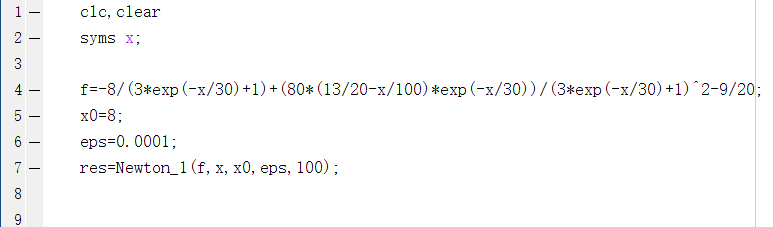
\includegraphics[scale=0.7]{figs/1(b)_1.jpg}
    }
    \hspace{0.1in}
    \subfigure[Function codes]{
        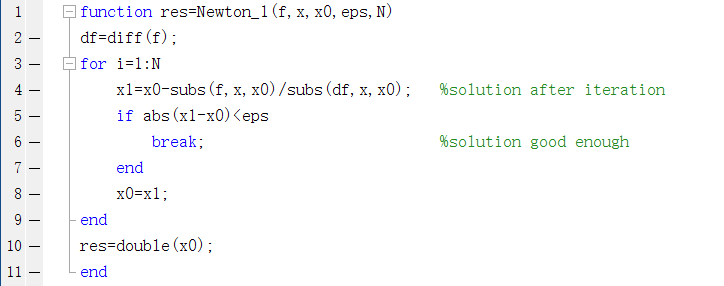
\includegraphics[scale=0.75]{figs/1(b)_2.jpg}        
    }
    \caption*{Two codes solving question (b) by Newton method of one-variable}
\end{figure}

\vspace{1em}
\hspace{-1.5em}{\bf Step 5. Answer the question}\par

We should hold the pigs for 12.3349 days, and then sell them to get the max profit which is 12.3349\$. 

\newpage

{\bf (c)}\par
Now we treat 800 as a new parameter $c$. 
The objective function becomes to
\begin{align*}
    f(x)=(0.65-0.01x)(\frac{c}{1+3e^{-\frac{x}{30}}})-0.45x
\end{align*}

And the differential of $f(x)$ becomes to 
\begin{align*}
    F=f'(x)=-\dfrac{c}{100\left(3\mathrm{e}^{-\frac{x}{30}}+1\right)}+\dfrac{c\cdot\left(\frac{13}{20}-\frac{x}{100}\right)\mathrm{e}^{-\frac{x}{30}}}{10{(3\mathrm{e}^{-\frac{x}{30}}+1)}^2}-0.45
\end{align*}

Since the sensitivity is about how effect the objective variables when the parameters change under 1\%, 
so we can let $c$ become 808, and calculate the time $t$ and the profit $P$. 
objective function $f(x)$ becomes
\begin{align*}
    f(x)=(0.65-0.01x)(\frac{808}{1+3e^{-\frac{x}{30}}})-0.45x
\end{align*}

And $x^*=12.3877, P^*=136.8334$, from the definition of sensitivity, the sensitivity is
\begin{align*}
    S(c,x)&=\frac{12.3877-12.3349}{12.3349}\cdot 100=0.428\\
    S(c,P)&=\frac{136.8334-135.4236}{135.4236}\cdot 100 =1.041
\end{align*}

We can also use Newton method to $F$ and find all optimal time $t$ and profit $P$ over 
$c\in [750:10:850]$. 

\begin{figure}[htbp]
    \centering
    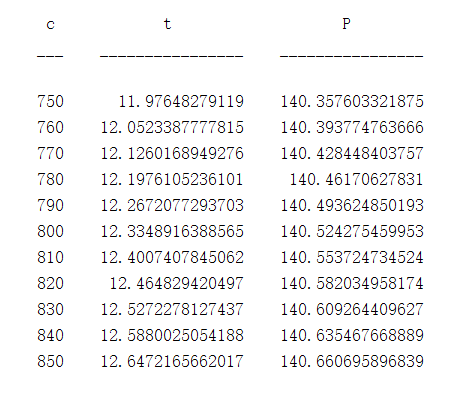
\includegraphics[scale=0.8]{figs/1(c)_1.jpg}
    \caption*{Sensitivity of final weight $c$, time $t$ and profit $P$}
\end{figure}

\begin{figure}[htbp]
    \centering
    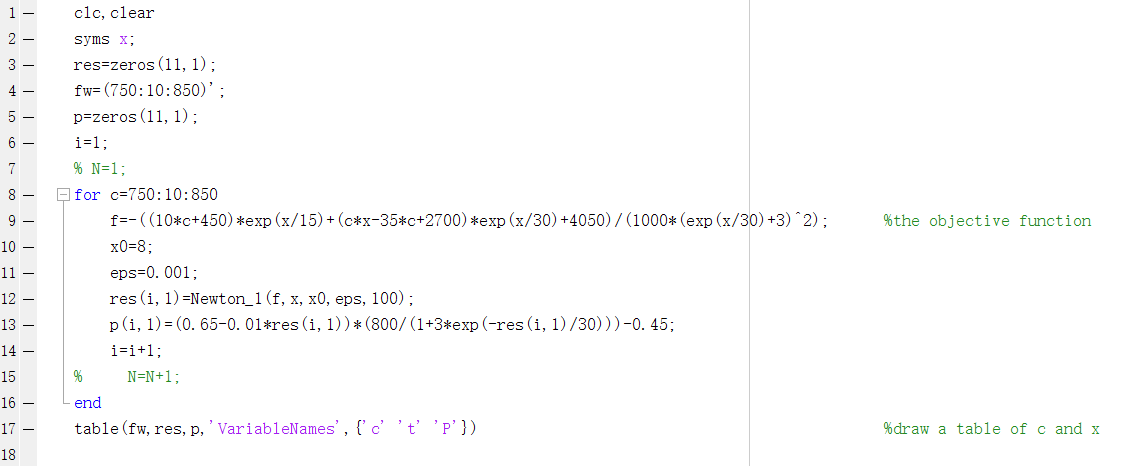
\includegraphics[scale=0.6]{figs/1(c)_2.jpg}
    \caption*{Codes in MATLAB}
\end{figure}

\newpage
\section*{\bf Question 6.from textbook}\par
{\bf (a)}

In the question 6, the response time relationship becomes to a linear relationship. 
Then let's apply the five-step method. 

\hspace{-1.5em}{\bf Step 1. Ask the question}\par 
There three stages in step 1. (Notice that $n$ and $t$ are matrices)

\vspace{0.5em}
\begin{tabular}{ll}
    {\bf Variables:}
    &$x$ = x-index of position\\
    &$y$ = y-index of potition\\
    &$n$ = average call times (times)\\
    &$t$ = each average response time (min)\\
    &$T$ = total average response time (min)\\
    {\bf Assumptions:}
    &$t = \vert x-x_0\vert +\vert y-y_0\vert$\\
    &$T=\frac{n\cdot t}{84}$\\
    &$0\leq x \leq 6, 0\leq y\leq 6$\\
    {\bf Objective:}
    &Minimize T
\end{tabular}

\vspace{1em}
\hspace{-1.5em}{\bf Step 2. Select the modeling approach}\par
In this question, we measure it as a multivariable unstrained optimization problem. 
If we solve it directly it would be very difficult since its objective function is very complicate. 
So we use random search model to solve it. 
Then it will become more easy. 

\vspace{1em}
\hspace{-1.5em}{\bf Step 3. Formulate the model}\par
The opitmal function $z=T$ is 
\begin{align*}
   z&=T\\
   &=(6(\lvert x-1\vert+\vert y-5\rvert)+8(\lvert x-3\vert+\vert y-5\rvert)+8(\lvert x-5\vert+\vert y-5\rvert)\\
   &\;\;\;+21(\lvert x-1\vert+\vert y-3\rvert)+6(\lvert x-3\vert+\vert y-3\rvert)+v3(\lvert x-5\vert+\vert y-3\rvert)\\
   &\;\;\;+18(\lvert x-1\vert+\vert y-1\rvert)+8(\lvert x-3\vert+\vert y-1\rvert)+6(\lvert x-5\vert+\vert y-1\rvert))/84
\end{align*}

\vspace{1em}
\hspace{-1.5em}{\bf Step 4. Solve the model}\par

Then we use random search method to solve this objective function. 
We set the boundary $x\in [0,6]$ and $y\in [0.6]$, and the iteration times becomes to 10000000. 
We can get the solution approaching to 
\begin{equation*}
    x_{\min}=1,\hspace{2em}
    y_{\min}=3,\hspace{2em}
    z_{\min}=2.6194
\end{equation*}

\vspace{1em}
\hspace{-1.5em}{\bf Step 5. Answer the question}\par

The optimal position to build the new facility is at position (1,3). 
Then the least average response time is 2.6194 minutes

\newpage
\begin{figure}[htbp]
    \centering
    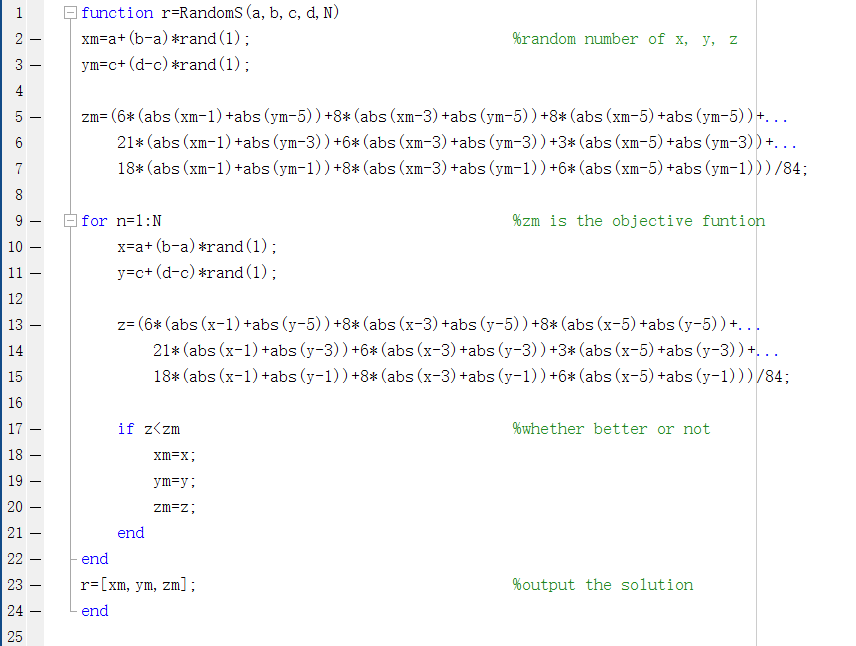
\includegraphics[scale=0.9]{figs/2_1.jpg}
    \caption*{Codes of question 6 in MATLAB}
\end{figure}

\end{spacing}
\end{document}